\documentclass[twoside]{book}

% Packages required by doxygen
\usepackage{fixltx2e}
\usepackage{calc}
\usepackage{doxygen}
\usepackage[export]{adjustbox} % also loads graphicx
\usepackage{graphicx}
\usepackage[utf8]{inputenc}
\usepackage{makeidx}
\usepackage{multicol}
\usepackage{multirow}
\PassOptionsToPackage{warn}{textcomp}
\usepackage{textcomp}
\usepackage[nointegrals]{wasysym}
\usepackage[table]{xcolor}

% Font selection
\usepackage[T1]{fontenc}
\usepackage[scaled=.90]{helvet}
\usepackage{courier}
\usepackage{amssymb}
\usepackage{sectsty}
\renewcommand{\familydefault}{\sfdefault}
\allsectionsfont{%
  \fontseries{bc}\selectfont%
  \color{darkgray}%
}
\renewcommand{\DoxyLabelFont}{%
  \fontseries{bc}\selectfont%
  \color{darkgray}%
}
\newcommand{\+}{\discretionary{\mbox{\scriptsize$\hookleftarrow$}}{}{}}

% Page & text layout
\usepackage{geometry}
\geometry{%
  a4paper,%
  top=2.5cm,%
  bottom=2.5cm,%
  left=2.5cm,%
  right=2.5cm%
}
\tolerance=750
\hfuzz=15pt
\hbadness=750
\setlength{\emergencystretch}{15pt}
\setlength{\parindent}{0cm}
\setlength{\parskip}{0.2cm}
\makeatletter
\renewcommand{\paragraph}{%
  \@startsection{paragraph}{4}{0ex}{-1.0ex}{1.0ex}{%
    \normalfont\normalsize\bfseries\SS@parafont%
  }%
}
\renewcommand{\subparagraph}{%
  \@startsection{subparagraph}{5}{0ex}{-1.0ex}{1.0ex}{%
    \normalfont\normalsize\bfseries\SS@subparafont%
  }%
}
\makeatother

% Headers & footers
\usepackage{fancyhdr}
\pagestyle{fancyplain}
\fancyhead[LE]{\fancyplain{}{\bfseries\thepage}}
\fancyhead[CE]{\fancyplain{}{}}
\fancyhead[RE]{\fancyplain{}{\bfseries\leftmark}}
\fancyhead[LO]{\fancyplain{}{\bfseries\rightmark}}
\fancyhead[CO]{\fancyplain{}{}}
\fancyhead[RO]{\fancyplain{}{\bfseries\thepage}}
\fancyfoot[LE]{\fancyplain{}{}}
\fancyfoot[CE]{\fancyplain{}{}}
\fancyfoot[RE]{\fancyplain{}{\bfseries\scriptsize Generated on Mon Sep 7 2015 10\+:26\+:49 for cnstr.\+me by Doxygen }}
\fancyfoot[LO]{\fancyplain{}{\bfseries\scriptsize Generated on Mon Sep 7 2015 10\+:26\+:49 for cnstr.\+me by Doxygen }}
\fancyfoot[CO]{\fancyplain{}{}}
\fancyfoot[RO]{\fancyplain{}{}}
\renewcommand{\footrulewidth}{0.4pt}
\renewcommand{\chaptermark}[1]{%
  \markboth{#1}{}%
}
\renewcommand{\sectionmark}[1]{%
  \markright{\thesection\ #1}%
}

% Indices & bibliography
\usepackage{natbib}
\usepackage[titles]{tocloft}
\setcounter{tocdepth}{3}
\setcounter{secnumdepth}{5}
\makeindex

% Hyperlinks (required, but should be loaded last)
\usepackage{ifpdf}
\ifpdf
  \usepackage[pdftex,pagebackref=true]{hyperref}
\else
  \usepackage[ps2pdf,pagebackref=true]{hyperref}
\fi
\hypersetup{%
  colorlinks=true,%
  linkcolor=blue,%
  citecolor=blue,%
  unicode%
}

% Custom commands
\newcommand{\clearemptydoublepage}{%
  \newpage{\pagestyle{empty}\cleardoublepage}%
}


%===== C O N T E N T S =====

\begin{document}

% Titlepage & ToC
\hypersetup{pageanchor=false,
             bookmarks=true,
             bookmarksnumbered=true,
             pdfencoding=unicode
            }
\pagenumbering{roman}
\begin{titlepage}
\vspace*{7cm}
\begin{center}%
{\Large cnstr.\+me }\\
\vspace*{1cm}
{\large Generated by Doxygen 1.8.10}\\
\vspace*{0.5cm}
{\small Mon Sep 7 2015 10:26:49}\\
\end{center}
\end{titlepage}
\clearemptydoublepage
\tableofcontents
\clearemptydoublepage
\pagenumbering{arabic}
\hypersetup{pageanchor=true}

%--- Begin generated contents ---
\chapter{Hierarchical Index}
\section{Class Hierarchy}
This inheritance list is sorted roughly, but not completely, alphabetically\+:\begin{DoxyCompactList}
\item \contentsline{section}{boton}{\pageref{classboton}}{}
\item \contentsline{section}{caja\+Anim}{\pageref{classcaja_anim}}{}
\item \contentsline{section}{caja\+Boton}{\pageref{classcaja_boton}}{}
\item \contentsline{section}{caja\+Gr\+Circulos}{\pageref{classcaja_gr_circulos}}{}
\item \contentsline{section}{caja\+Imagen}{\pageref{classcaja_imagen}}{}
\item \contentsline{section}{caja\+Texto}{\pageref{classcaja_texto}}{}
\item \contentsline{section}{Contenedor}{\pageref{class_contenedor}}{}
\item \contentsline{section}{Eventos}{\pageref{class_eventos}}{}
\item \contentsline{section}{Galeria}{\pageref{class_galeria}}{}
\item \contentsline{section}{gestor3\+D}{\pageref{classgestor3_d}}{}
\item \contentsline{section}{Globales}{\pageref{class_globales}}{}
\item \contentsline{section}{Grid}{\pageref{class_grid}}{}
\item \contentsline{section}{Gui\+Escenas}{\pageref{class_gui_escenas}}{}
\item \contentsline{section}{Loop}{\pageref{class_loop}}{}
\item of\+Base\+App\begin{DoxyCompactList}
\item \contentsline{section}{of\+App}{\pageref{classof_app}}{}
\item \contentsline{section}{of\+App}{\pageref{classof_app}}{}
\end{DoxyCompactList}
\item \contentsline{section}{Principal}{\pageref{class_principal}}{}
\item \contentsline{section}{Rafaga}{\pageref{class_rafaga}}{}
\item \contentsline{section}{Titulo}{\pageref{class_titulo}}{}
\end{DoxyCompactList}

\chapter{Class Index}
\section{Class List}
Here are the classes, structs, unions and interfaces with brief descriptions\+:\begin{DoxyCompactList}
\item\contentsline{section}{\hyperlink{classboton}{boton} }{\pageref{classboton}}{}
\item\contentsline{section}{\hyperlink{classcaja_anim}{caja\+Anim} }{\pageref{classcaja_anim}}{}
\item\contentsline{section}{\hyperlink{classcaja_boton}{caja\+Boton} }{\pageref{classcaja_boton}}{}
\item\contentsline{section}{\hyperlink{classcaja_gr_circulos}{caja\+Gr\+Circulos} }{\pageref{classcaja_gr_circulos}}{}
\item\contentsline{section}{\hyperlink{classcaja_imagen}{caja\+Imagen} }{\pageref{classcaja_imagen}}{}
\item\contentsline{section}{\hyperlink{classcaja_texto}{caja\+Texto} }{\pageref{classcaja_texto}}{}
\item\contentsline{section}{\hyperlink{class_contenedor}{Contenedor} }{\pageref{class_contenedor}}{}
\item\contentsline{section}{\hyperlink{class_eventos}{Eventos} }{\pageref{class_eventos}}{}
\item\contentsline{section}{\hyperlink{class_galeria}{Galeria} }{\pageref{class_galeria}}{}
\item\contentsline{section}{\hyperlink{classgestor3_d}{gestor3\+D} }{\pageref{classgestor3_d}}{}
\item\contentsline{section}{\hyperlink{class_globales}{Globales} }{\pageref{class_globales}}{}
\item\contentsline{section}{\hyperlink{class_grid}{Grid} }{\pageref{class_grid}}{}
\item\contentsline{section}{\hyperlink{class_gui_escenas}{Gui\+Escenas} }{\pageref{class_gui_escenas}}{}
\item\contentsline{section}{\hyperlink{class_loop}{Loop} }{\pageref{class_loop}}{}
\item\contentsline{section}{\hyperlink{classof_app}{of\+App} }{\pageref{classof_app}}{}
\item\contentsline{section}{\hyperlink{class_principal}{Principal} }{\pageref{class_principal}}{}
\item\contentsline{section}{\hyperlink{class_rafaga}{Rafaga} }{\pageref{class_rafaga}}{}
\item\contentsline{section}{\hyperlink{class_titulo}{Titulo} }{\pageref{class_titulo}}{}
\end{DoxyCompactList}

\chapter{Class Documentation}
\hypertarget{classboton}{}\section{boton Class Reference}
\label{classboton}\index{boton@{boton}}
\subsection*{Public Types}
\begin{DoxyCompactItemize}
\item 
\hypertarget{classboton_a62def824d19d57b2180e1539e573f906}{}enum {\bfseries tipos\+Botones} \{ {\bfseries circulo\+Texto}, 
{\bfseries circulo\+Imagen}, 
{\bfseries rect\+Texto}, 
{\bfseries rect\+Imagen}
 \}\label{classboton_a62def824d19d57b2180e1539e573f906}

\end{DoxyCompactItemize}
\subsection*{Public Member Functions}
\begin{DoxyCompactItemize}
\item 
\hypertarget{classboton_a3372383d8b639a7f900ffad42a81f575}{}{\bfseries boton} (tipos\+Botones \+\_\+tipo\+Btn, string \+\_\+color\+Boton)\label{classboton_a3372383d8b639a7f900ffad42a81f575}

\item 
\hypertarget{classboton_a358ea773863186635746810589c3d275}{}void {\bfseries update} (int, int)\label{classboton_a358ea773863186635746810589c3d275}

\item 
\hypertarget{classboton_a564fb8db709acbb55fa8dbd6fee7ff8a}{}void {\bfseries draw} (of\+Vec2f, int, string)\label{classboton_a564fb8db709acbb55fa8dbd6fee7ff8a}

\item 
\hypertarget{classboton_a02b7a19feae6df824d68f134fce6dab0}{}void {\bfseries draw} (of\+Vec2f, int, int, string)\label{classboton_a02b7a19feae6df824d68f134fce6dab0}

\item 
\hypertarget{classboton_a297b08b9c3935c4cd55628c7bbdc5876}{}void {\bfseries draw} (of\+Vec2f, int, of\+Image)\label{classboton_a297b08b9c3935c4cd55628c7bbdc5876}

\item 
\hypertarget{classboton_a5b5786e0e80df5c94c04e607e16920e7}{}void {\bfseries draw} (of\+Vec2f, int, int, of\+Image)\label{classboton_a5b5786e0e80df5c94c04e607e16920e7}

\item 
\hypertarget{classboton_ab7d750781870e9c71f3fdfd8da457c06}{}void {\bfseries mouse\+Moved} (of\+Mouse\+Event\+Args \&args)\label{classboton_ab7d750781870e9c71f3fdfd8da457c06}

\item 
\hypertarget{classboton_ac9791d558f667d015e0e3913b6162a66}{}void {\bfseries mouse\+Dragged} (of\+Mouse\+Event\+Args \&args)\label{classboton_ac9791d558f667d015e0e3913b6162a66}

\item 
\hypertarget{classboton_a7ae6e9bfc79c27b6f0727898fb572e60}{}void {\bfseries mouse\+Pressed} (of\+Mouse\+Event\+Args \&args)\label{classboton_a7ae6e9bfc79c27b6f0727898fb572e60}

\item 
\hypertarget{classboton_a453f2c190a1f4d8a39d7ada30d78f8fd}{}void {\bfseries mouse\+Released} (of\+Mouse\+Event\+Args \&args)\label{classboton_a453f2c190a1f4d8a39d7ada30d78f8fd}

\item 
\hypertarget{classboton_a2fb4e81bea8fb4367b7dc5c2e97a747b}{}bool {\bfseries dentro} (float, float)\label{classboton_a2fb4e81bea8fb4367b7dc5c2e97a747b}

\item 
\hypertarget{classboton_aaeaf90d2c85588fa211476a02216d812}{}void {\bfseries estados} (bool)\label{classboton_aaeaf90d2c85588fa211476a02216d812}

\item 
\hypertarget{classboton_a11764cdbb4e87c91f9d25c604fba8371}{}bool {\bfseries getter} ()\label{classboton_a11764cdbb4e87c91f9d25c604fba8371}

\item 
\hypertarget{classboton_aff539a42864d6fcba24af7e2ae8cb734}{}void {\bfseries setter} (bool \+\_\+dentro)\label{classboton_aff539a42864d6fcba24af7e2ae8cb734}

\end{DoxyCompactItemize}
\subsection*{Public Attributes}
\begin{DoxyCompactItemize}
\item 
\hypertarget{classboton_acd7f66034efc19d87cab127c540a75da}{}of\+Event$<$ string $>$ {\bfseries evento}\label{classboton_acd7f66034efc19d87cab127c540a75da}

\item 
\hypertarget{classboton_a944bd8256ae5c050786a562eeb725f80}{}string {\bfseries color\+Boton}\label{classboton_a944bd8256ae5c050786a562eeb725f80}

\item 
\hypertarget{classboton_a765cc553638925511282f64dbfffeee9}{}string {\bfseries texto}\label{classboton_a765cc553638925511282f64dbfffeee9}

\item 
\hypertarget{classboton_a460d5390561a0d2da31462c25912afc9}{}tipos\+Botones {\bfseries tipo\+Boton}\label{classboton_a460d5390561a0d2da31462c25912afc9}

\end{DoxyCompactItemize}


The documentation for this class was generated from the following files\+:\begin{DoxyCompactItemize}
\item 
src/\+Gui/Boton.\+h\item 
src/\+Gui/Boton.\+cpp\end{DoxyCompactItemize}

\hypertarget{classcaja_anim}{}\section{caja\+Anim Class Reference}
\label{classcaja_anim}\index{caja\+Anim@{caja\+Anim}}
\subsection*{Public Member Functions}
\begin{DoxyCompactItemize}
\item 
\hyperlink{classcaja_anim_a80adf751100761f379a05069a2d2698c}{caja\+Anim} (int, int, of\+Video\+Player)
\item 
void \hyperlink{classcaja_anim_aaa5cf076d2b84a1def47134500f695e7}{draw} ()
\item 
void \hyperlink{classcaja_anim_a375bf7404927f84b5896d5b04f79ee5d}{update} ()
\end{DoxyCompactItemize}
\subsection*{Public Attributes}
\begin{DoxyCompactItemize}
\item 
of\+Fbo \hyperlink{classcaja_anim_a1b412216eb252618f429414692b4ee60}{fbo}
\item 
of\+Video\+Player \hyperlink{classcaja_anim_a0fd4a41de88a6950430b437f600029f9}{video}
\end{DoxyCompactItemize}


\subsection{Constructor \& Destructor Documentation}
\hypertarget{classcaja_anim_a80adf751100761f379a05069a2d2698c}{}\index{caja\+Anim@{caja\+Anim}!caja\+Anim@{caja\+Anim}}
\index{caja\+Anim@{caja\+Anim}!caja\+Anim@{caja\+Anim}}
\subsubsection[{caja\+Anim(int, int, of\+Video\+Player)}]{\setlength{\rightskip}{0pt plus 5cm}caja\+Anim\+::caja\+Anim (
\begin{DoxyParamCaption}
\item[{int}]{\+\_\+largo, }
\item[{int}]{\+\_\+ancho, }
\item[{of\+Video\+Player}]{\+\_\+video}
\end{DoxyParamCaption}
)}\label{classcaja_anim_a80adf751100761f379a05069a2d2698c}
constructor \hyperlink{classcaja_anim}{caja\+Anim} 
\begin{DoxyParams}{Parameters}
{\em (posx,posy,video} & ya cargado desde load) \\
\hline
\end{DoxyParams}


\subsection{Member Function Documentation}
\hypertarget{classcaja_anim_aaa5cf076d2b84a1def47134500f695e7}{}\index{caja\+Anim@{caja\+Anim}!draw@{draw}}
\index{draw@{draw}!caja\+Anim@{caja\+Anim}}
\subsubsection[{draw()}]{\setlength{\rightskip}{0pt plus 5cm}void caja\+Anim\+::draw (
\begin{DoxyParamCaption}
{}
\end{DoxyParamCaption}
)}\label{classcaja_anim_aaa5cf076d2b84a1def47134500f695e7}
dibuja la caja dentro del fbo \hypertarget{classcaja_anim_a375bf7404927f84b5896d5b04f79ee5d}{}\index{caja\+Anim@{caja\+Anim}!update@{update}}
\index{update@{update}!caja\+Anim@{caja\+Anim}}
\subsubsection[{update()}]{\setlength{\rightskip}{0pt plus 5cm}void caja\+Anim\+::update (
\begin{DoxyParamCaption}
{}
\end{DoxyParamCaption}
)}\label{classcaja_anim_a375bf7404927f84b5896d5b04f79ee5d}
colocar siempre en update de escena para refrescar video 

\subsection{Member Data Documentation}
\hypertarget{classcaja_anim_a1b412216eb252618f429414692b4ee60}{}\index{caja\+Anim@{caja\+Anim}!fbo@{fbo}}
\index{fbo@{fbo}!caja\+Anim@{caja\+Anim}}
\subsubsection[{fbo}]{\setlength{\rightskip}{0pt plus 5cm}of\+Fbo caja\+Anim\+::fbo}\label{classcaja_anim_a1b412216eb252618f429414692b4ee60}
regresa F\+B\+O del v�deo \begin{DoxyReturn}{Returns}
devuelve fbo 
\end{DoxyReturn}
\hypertarget{classcaja_anim_a0fd4a41de88a6950430b437f600029f9}{}\index{caja\+Anim@{caja\+Anim}!video@{video}}
\index{video@{video}!caja\+Anim@{caja\+Anim}}
\subsubsection[{video}]{\setlength{\rightskip}{0pt plus 5cm}of\+Video\+Player caja\+Anim\+::video}\label{classcaja_anim_a0fd4a41de88a6950430b437f600029f9}
se debe acceder para poder modificar sus propiedades \begin{DoxyReturn}{Returns}
devuelve el video tipo of\+Video\+Player 
\end{DoxyReturn}


The documentation for this class was generated from the following files\+:\begin{DoxyCompactItemize}
\item 
src/\+Cajas/caja\+Anim.\+h\item 
src/\+Cajas/caja\+Anim.\+cpp\end{DoxyCompactItemize}

\hypertarget{classcaja_boton}{}\section{caja\+Boton Class Reference}
\label{classcaja_boton}\index{caja\+Boton@{caja\+Boton}}
\subsection*{Public Member Functions}
\begin{DoxyCompactItemize}
\item 
\hypertarget{classcaja_boton_a989e25ba5f2e1a250034d22aabdefe30}{}{\bfseries caja\+Boton} (unsigned int \+\_\+pos\+Fila, int \+\_\+w, int \+\_\+h, int \+\_\+radio, string \+\_\+titulo, boton\+::tipos\+Botones \+\_\+tipo\+Btn, string \+\_\+color\+Btn)\label{classcaja_boton_a989e25ba5f2e1a250034d22aabdefe30}

\item 
\hypertarget{classcaja_boton_a216275f9afe007fcb60d48ed899bad41}{}{\bfseries caja\+Boton} (unsigned int \+\_\+pos\+Fila, int \+\_\+w, int \+\_\+h, string \+\_\+titulo, \hyperlink{classboton}{boton} \+\_\+btn)\label{classcaja_boton_a216275f9afe007fcb60d48ed899bad41}

\item 
\hypertarget{classcaja_boton_abfaf12f5807f22b90143442ae896afcd}{}void {\bfseries draw} (int, int)\label{classcaja_boton_abfaf12f5807f22b90143442ae896afcd}

\item 
\hypertarget{classcaja_boton_a37cb1ba617e40e4140b079a87fcb239a}{}void {\bfseries update} (int, int)\label{classcaja_boton_a37cb1ba617e40e4140b079a87fcb239a}

\item 
\hypertarget{classcaja_boton_ab51fcdb3e4762a6add779f09ce4c2cb7}{}void {\bfseries estados} (bool)\label{classcaja_boton_ab51fcdb3e4762a6add779f09ce4c2cb7}

\end{DoxyCompactItemize}
\subsection*{Public Attributes}
\begin{DoxyCompactItemize}
\item 
\hypertarget{classcaja_boton_a67f70e9feed641b60d25ae1dc1ecdf8c}{}\hyperlink{classboton}{boton} {\bfseries btn}\label{classcaja_boton_a67f70e9feed641b60d25ae1dc1ecdf8c}

\item 
\hypertarget{classcaja_boton_ad8c5f144b388b71a27c6f0692fe40da7}{}int {\bfseries h}\label{classcaja_boton_ad8c5f144b388b71a27c6f0692fe40da7}

\item 
\hypertarget{classcaja_boton_aa8688048b1688c0076235424d3c7b625}{}unsigned int {\bfseries pos\+Fila}\label{classcaja_boton_aa8688048b1688c0076235424d3c7b625}

\item 
\hypertarget{classcaja_boton_a31225c139dfe4c239b35fcd5ef099d03}{}string {\bfseries id}\label{classcaja_boton_a31225c139dfe4c239b35fcd5ef099d03}

\end{DoxyCompactItemize}


The documentation for this class was generated from the following files\+:\begin{DoxyCompactItemize}
\item 
src/\+Cajas/caja\+Boton.\+h\item 
src/\+Cajas/caja\+Boton.\+cpp\end{DoxyCompactItemize}

\hypertarget{classcaja_gr_circulos}{}\section{caja\+Gr\+Circulos Class Reference}
\label{classcaja_gr_circulos}\index{caja\+Gr\+Circulos@{caja\+Gr\+Circulos}}
\subsection*{Public Member Functions}
\begin{DoxyCompactItemize}
\item 
\hyperlink{classcaja_gr_circulos_a54ebb2fafbbc7bd4aa13d934d52040a7}{caja\+Gr\+Circulos} (unsigned int \+\_\+pos\+Fila, int \+\_\+w, int \+\_\+h, float \+\_\+v\+Max, float \+\_\+v\+Final, float \+\_\+escala\+Circulo=0.\+8, float \+\_\+escala\+Interior=0.\+9, of\+Color=of\+Color\+::white, of\+Color=of\+Color\+::light\+Gray)
\item 
\hypertarget{classcaja_gr_circulos_af5b406775d6dc3d4226614bd13920b91}{}void {\bfseries draw} ()\label{classcaja_gr_circulos_af5b406775d6dc3d4226614bd13920b91}

\item 
\hypertarget{classcaja_gr_circulos_a5bf88c348cc168c6c1dfbb113c258a98}{}void {\bfseries inicia\+Anim} ()\label{classcaja_gr_circulos_a5bf88c348cc168c6c1dfbb113c258a98}

\item 
\hypertarget{classcaja_gr_circulos_ad1a0f47dc0a6a7eb52acbc5ddb530587}{}void {\bfseries update} ()\label{classcaja_gr_circulos_ad1a0f47dc0a6a7eb52acbc5ddb530587}

\end{DoxyCompactItemize}
\subsection*{Public Attributes}
\begin{DoxyCompactItemize}
\item 
\hypertarget{classcaja_gr_circulos_ac98d0dd84d7c3bf01515a2105aa94ca6}{}of\+Fbo {\bfseries fbo}\label{classcaja_gr_circulos_ac98d0dd84d7c3bf01515a2105aa94ca6}

\item 
\hypertarget{classcaja_gr_circulos_a1a43900aefa7e2d6023448248cf71620}{}int {\bfseries h}\label{classcaja_gr_circulos_a1a43900aefa7e2d6023448248cf71620}

\item 
\hypertarget{classcaja_gr_circulos_ad08d9eda45829153965ed1cc4e45e1c2}{}unsigned int {\bfseries pos\+Fila}\label{classcaja_gr_circulos_ad08d9eda45829153965ed1cc4e45e1c2}

\end{DoxyCompactItemize}


\subsection{Constructor \& Destructor Documentation}
\hypertarget{classcaja_gr_circulos_a54ebb2fafbbc7bd4aa13d934d52040a7}{}\index{caja\+Gr\+Circulos@{caja\+Gr\+Circulos}!caja\+Gr\+Circulos@{caja\+Gr\+Circulos}}
\index{caja\+Gr\+Circulos@{caja\+Gr\+Circulos}!caja\+Gr\+Circulos@{caja\+Gr\+Circulos}}
\subsubsection[{caja\+Gr\+Circulos(unsigned int \+\_\+pos\+Fila, int \+\_\+w, int \+\_\+h, float \+\_\+v\+Max, float \+\_\+v\+Final, float \+\_\+escala\+Circulo=0.\+8, float \+\_\+escala\+Interior=0.\+9, of\+Color=of\+Color\+::white, of\+Color=of\+Color\+::light\+Gray)}]{\setlength{\rightskip}{0pt plus 5cm}caja\+Gr\+Circulos\+::caja\+Gr\+Circulos (
\begin{DoxyParamCaption}
\item[{unsigned int}]{\+\_\+pos\+Fila, }
\item[{int}]{\+\_\+w, }
\item[{int}]{\+\_\+h, }
\item[{float}]{\+\_\+v\+Max, }
\item[{float}]{\+\_\+v\+Final, }
\item[{float}]{\+\_\+escala\+Circulo = {\ttfamily 0.8}, }
\item[{float}]{\+\_\+escala\+Interior = {\ttfamily 0.9}, }
\item[{of\+Color}]{\+\_\+bg = {\ttfamily ofColor\+:\+:white}, }
\item[{of\+Color}]{\+\_\+fg = {\ttfamily ofColor\+:\+:lightGray}}
\end{DoxyParamCaption}
)}\label{classcaja_gr_circulos_a54ebb2fafbbc7bd4aa13d934d52040a7}
parametros 
\begin{DoxyParams}{Parameters}
{\em posicion} & de arriba a abajo en el contenedor \\
\hline
{\em largo} & y ancho para fbo.\+allocate \\
\hline
{\em Valor} & maximo del arco (coincide con los 360 grados) \\
\hline
{\em valor} & que se desea mostrar \\
\hline
{\em escala\+Circulo} & relativo a la caja (0.\+8 por defecto) \\
\hline
{\em escala\+Circulo} & interior relativo a la caja (0.\+9 por defecto) \\
\hline
{\em color} & de fondo (white por defecto) \\
\hline
{\em color} & de la barra (ligth\+Gray por defecto) \\
\hline
\end{DoxyParams}


The documentation for this class was generated from the following files\+:\begin{DoxyCompactItemize}
\item 
src/\+Cajas/caja\+G\+R\+\_\+\+Circulos.\+h\item 
src/\+Cajas/caja\+G\+R\+\_\+\+Circulos.\+cpp\end{DoxyCompactItemize}

\hypertarget{classcaja_imagen}{}\section{caja\+Imagen Class Reference}
\label{classcaja_imagen}\index{caja\+Imagen@{caja\+Imagen}}
\subsection*{Public Member Functions}
\begin{DoxyCompactItemize}
\item 
\hyperlink{classcaja_imagen_a57428676967a129015865f8f912aab10}{caja\+Imagen} (int, int, of\+Image, unsigned int)
\item 
\hypertarget{classcaja_imagen_af9b623ccda2a4d034b9bd3690e897696}{}void {\bfseries draw} ()\label{classcaja_imagen_af9b623ccda2a4d034b9bd3690e897696}

\item 
\hypertarget{classcaja_imagen_a5621901b1f210fb1119447d06412fe9d}{}void {\bfseries update} ()\label{classcaja_imagen_a5621901b1f210fb1119447d06412fe9d}

\item 
\hypertarget{classcaja_imagen_a6d3ded7d688db251527244dc5fd75b33}{}void {\bfseries estados} (bool)\label{classcaja_imagen_a6d3ded7d688db251527244dc5fd75b33}

\end{DoxyCompactItemize}
\subsection*{Public Attributes}
\begin{DoxyCompactItemize}
\item 
\hypertarget{classcaja_imagen_ad808c69c58b0df75b0bd6c5c5c6d4f63}{}string {\bfseries texto}\label{classcaja_imagen_ad808c69c58b0df75b0bd6c5c5c6d4f63}

\item 
\hypertarget{classcaja_imagen_ac3f8b1f8df6b6a5c31bd7b09519c1d6f}{}of\+Fbo {\bfseries fbo}\label{classcaja_imagen_ac3f8b1f8df6b6a5c31bd7b09519c1d6f}

\item 
\hypertarget{classcaja_imagen_ae057d8d84b7f0cbacbd44d080e2dd1a7}{}of\+Image {\bfseries imagen}\label{classcaja_imagen_ae057d8d84b7f0cbacbd44d080e2dd1a7}

\item 
\hypertarget{classcaja_imagen_affca2df82f3ccedcba990f8473c5590e}{}int {\bfseries h}\label{classcaja_imagen_affca2df82f3ccedcba990f8473c5590e}

\item 
\hypertarget{classcaja_imagen_a6cf502995edfc720f7cc88f51b8a5d1a}{}unsigned int {\bfseries pos\+Fila}\label{classcaja_imagen_a6cf502995edfc720f7cc88f51b8a5d1a}

\end{DoxyCompactItemize}


\subsection{Constructor \& Destructor Documentation}
\hypertarget{classcaja_imagen_a57428676967a129015865f8f912aab10}{}\index{caja\+Imagen@{caja\+Imagen}!caja\+Imagen@{caja\+Imagen}}
\index{caja\+Imagen@{caja\+Imagen}!caja\+Imagen@{caja\+Imagen}}
\subsubsection[{caja\+Imagen(int, int, of\+Image, unsigned int)}]{\setlength{\rightskip}{0pt plus 5cm}caja\+Imagen\+::caja\+Imagen (
\begin{DoxyParamCaption}
\item[{int}]{\+\_\+largo, }
\item[{int}]{\+\_\+ancho, }
\item[{of\+Image}]{\+\_\+textura, }
\item[{unsigned int}]{\+\_\+pos\+Fila}
\end{DoxyParamCaption}
)}\label{classcaja_imagen_a57428676967a129015865f8f912aab10}
Par�metros 
\begin{DoxyParams}{Parameters}
{\em ancho} & y largo para allocate del fbo \\
\hline
{\em textura} & a insertar en fbo \\
\hline
{\em posicion} & de arriba a abajo en contenedor \\
\hline
\end{DoxyParams}


The documentation for this class was generated from the following files\+:\begin{DoxyCompactItemize}
\item 
src/\+Cajas/caja\+Imagen.\+h\item 
src/\+Cajas/caja\+Imagen.\+cpp\end{DoxyCompactItemize}

\hypertarget{classcaja_texto}{}\section{caja\+Texto Class Reference}
\label{classcaja_texto}\index{caja\+Texto@{caja\+Texto}}
\subsection*{Public Member Functions}
\begin{DoxyCompactItemize}
\item 
\hyperlink{classcaja_texto_a5321f70b574412666cc6b05699e5dae9}{caja\+Texto} (unsigned int, int, int, string, of\+Color, of\+Color)
\item 
\hypertarget{classcaja_texto_a5bc02d7f55e12fd32715e4509853a558}{}void {\bfseries draw} ()\label{classcaja_texto_a5bc02d7f55e12fd32715e4509853a558}

\item 
\hypertarget{classcaja_texto_a3c18217bfbc1508e94d43e79864451a1}{}void {\bfseries update} ()\label{classcaja_texto_a3c18217bfbc1508e94d43e79864451a1}

\item 
\hypertarget{classcaja_texto_a4478fed316945d70b7c22c3a644dd3f8}{}void {\bfseries estados} (bool)\label{classcaja_texto_a4478fed316945d70b7c22c3a644dd3f8}

\end{DoxyCompactItemize}
\subsection*{Public Attributes}
\begin{DoxyCompactItemize}
\item 
\hypertarget{classcaja_texto_ad93c32582acc4ef10d27fe572d140404}{}of\+Fbo {\bfseries fbo}\label{classcaja_texto_ad93c32582acc4ef10d27fe572d140404}

\item 
\hypertarget{classcaja_texto_ac0008cf847065d4e704cc0ba6dee9a83}{}int {\bfseries h}\label{classcaja_texto_ac0008cf847065d4e704cc0ba6dee9a83}

\item 
\hypertarget{classcaja_texto_a9510a1d9eccb62c787c9c2dca96689ba}{}unsigned int {\bfseries pos\+Fila}\label{classcaja_texto_a9510a1d9eccb62c787c9c2dca96689ba}

\end{DoxyCompactItemize}


\subsection{Constructor \& Destructor Documentation}
\hypertarget{classcaja_texto_a5321f70b574412666cc6b05699e5dae9}{}\index{caja\+Texto@{caja\+Texto}!caja\+Texto@{caja\+Texto}}
\index{caja\+Texto@{caja\+Texto}!caja\+Texto@{caja\+Texto}}
\subsubsection[{caja\+Texto(unsigned int, int, int, string, of\+Color, of\+Color)}]{\setlength{\rightskip}{0pt plus 5cm}caja\+Texto\+::caja\+Texto (
\begin{DoxyParamCaption}
\item[{unsigned int}]{\+\_\+pos\+Fila, }
\item[{int}]{\+\_\+largo, }
\item[{int}]{\+\_\+ancho, }
\item[{string}]{\+\_\+texto, }
\item[{of\+Color}]{\+\_\+color\+Fondo, }
\item[{of\+Color}]{\+\_\+color\+Texto}
\end{DoxyParamCaption}
)}\label{classcaja_texto_a5321f70b574412666cc6b05699e5dae9}
par�metros de entrada 
\begin{DoxyParams}{Parameters}
{\em ancho} & y largo para allocate \\
\hline
{\em texto} & a mostrar \\
\hline
{\em color} & de fondo \\
\hline
{\em color} & de texto \\
\hline
{\em orden} & de arriba a abajo en contenedor \\
\hline
\end{DoxyParams}


The documentation for this class was generated from the following files\+:\begin{DoxyCompactItemize}
\item 
src/\+Cajas/caja\+Texto.\+h\item 
src/\+Cajas/caja\+Texto.\+cpp\end{DoxyCompactItemize}

\hypertarget{class_contenedor}{}\section{Contenedor Class Reference}
\label{class_contenedor}\index{Contenedor@{Contenedor}}
\subsection*{Public Member Functions}
\begin{DoxyCompactItemize}
\item 
void \hyperlink{class_contenedor_aa208cc46b9d2bc97de702ac05279f41a}{setup} (int, int, string, bool, bool)
\item 
\hypertarget{class_contenedor_a3a37a7e965501d9011809929c86ad4ec}{}void {\bfseries draw} (int, int)\label{class_contenedor_a3a37a7e965501d9011809929c86ad4ec}

\item 
\hypertarget{class_contenedor_a72d6fc0022b74a22f256963a7e2e3e91}{}void {\bfseries update} ()\label{class_contenedor_a72d6fc0022b74a22f256963a7e2e3e91}

\item 
\hypertarget{class_contenedor_a66d32b54802e34352cc9e41a84b88e3f}{}void {\bfseries estados} (bool)\label{class_contenedor_a66d32b54802e34352cc9e41a84b88e3f}

\item 
\hypertarget{class_contenedor_a9a1499d5675f56eb82121e1c437f3928}{}void {\bfseries animacion} ()\label{class_contenedor_a9a1499d5675f56eb82121e1c437f3928}

\item 
void \hyperlink{class_contenedor_a6a554a96c28850594c5e8c4e5479d0f5}{fila} (\hyperlink{classcaja_gr_circulos}{caja\+Gr\+Circulos})
\item 
\hypertarget{class_contenedor_ac6e4cb9f390ef9fc8ecedda28bc069d3}{}void {\bfseries fila} (\hyperlink{classcaja_texto}{caja\+Texto})\label{class_contenedor_ac6e4cb9f390ef9fc8ecedda28bc069d3}

\item 
\hypertarget{class_contenedor_aa1db23dbedc3d235007e2d94d8f60e72}{}void {\bfseries fila} (\hyperlink{classcaja_imagen}{caja\+Imagen})\label{class_contenedor_aa1db23dbedc3d235007e2d94d8f60e72}

\item 
\hypertarget{class_contenedor_ad9b5790fbd88789c8a0ee2a119f213e6}{}void {\bfseries fila} (\hyperlink{classcaja_boton}{caja\+Boton})\label{class_contenedor_ad9b5790fbd88789c8a0ee2a119f213e6}

\item 
\hypertarget{class_contenedor_a7194aa7dca505dcbce9f9361e6c76b5d}{}void {\bfseries mouse\+Moved} (of\+Mouse\+Event\+Args \&args)\label{class_contenedor_a7194aa7dca505dcbce9f9361e6c76b5d}

\item 
\hypertarget{class_contenedor_a2da02e658ff662b3f2e719ec3c99919f}{}void {\bfseries mouse\+Dragged} (of\+Mouse\+Event\+Args \&args)\label{class_contenedor_a2da02e658ff662b3f2e719ec3c99919f}

\item 
\hypertarget{class_contenedor_aeff7750963999f99d04efce501a6dd65}{}void {\bfseries mouse\+Pressed} (of\+Mouse\+Event\+Args \&args)\label{class_contenedor_aeff7750963999f99d04efce501a6dd65}

\item 
\hypertarget{class_contenedor_ad1a27b53a72b784e13ae5b8e19714889}{}void {\bfseries mouse\+Released} (of\+Mouse\+Event\+Args \&args)\label{class_contenedor_ad1a27b53a72b784e13ae5b8e19714889}

\item 
\hypertarget{class_contenedor_ae6c8c66a94b7e3b862dc4a4543d8aab4}{}bool {\bfseries dentro} (float, float)\label{class_contenedor_ae6c8c66a94b7e3b862dc4a4543d8aab4}

\item 
\hypertarget{class_contenedor_aed519fcfe3ea010d9aabf41147556f64}{}bool {\bfseries getter} ()\label{class_contenedor_aed519fcfe3ea010d9aabf41147556f64}

\item 
\hypertarget{class_contenedor_a6091fd94668f43b2941bb215f4ca1056}{}void {\bfseries setter} (bool)\label{class_contenedor_a6091fd94668f43b2941bb215f4ca1056}

\end{DoxyCompactItemize}
\subsection*{Public Attributes}
\begin{DoxyCompactItemize}
\item 
\hypertarget{class_contenedor_a9954785d005a73707c436e56c2a756b5}{}map$<$ string, \hyperlink{classcaja_boton}{caja\+Boton} $>$ {\bfseries cajas\+Botones}\label{class_contenedor_a9954785d005a73707c436e56c2a756b5}

\item 
\hypertarget{class_contenedor_aa2768c25738e679011c023a6717db5da}{}vector$<$ of\+Fbo $>$ {\bfseries filas}\label{class_contenedor_aa2768c25738e679011c023a6717db5da}

\item 
\hypertarget{class_contenedor_a839d9dbaa48672ff53177a2feaa8f9d1}{}int {\bfseries largo}\label{class_contenedor_a839d9dbaa48672ff53177a2feaa8f9d1}

\item 
\hypertarget{class_contenedor_accfb6bb135cd4045cbc875350b46c981}{}int {\bfseries ancho\+Final}\label{class_contenedor_accfb6bb135cd4045cbc875350b46c981}

\item 
\hypertarget{class_contenedor_a9e2a7cc2206db8a8413558be324bb270}{}\hyperlink{classboton}{boton} {\bfseries boton\+Salir}\label{class_contenedor_a9e2a7cc2206db8a8413558be324bb270}

\item 
\hypertarget{class_contenedor_a06e4ecc3563676436e7b5209eeeeaaa2}{}of\+True\+Type\+Font {\bfseries titulo}\label{class_contenedor_a06e4ecc3563676436e7b5209eeeeaaa2}

\item 
\hypertarget{class_contenedor_a905a163b3e98855a3cae2b45380fb37f}{}string {\bfseries texto\+Titulo}\label{class_contenedor_a905a163b3e98855a3cae2b45380fb37f}

\item 
\hypertarget{class_contenedor_a0d7e72e35e93257544a5482fdb2cd2da}{}ofx\+Tween {\bfseries animacion\+Contenedor}\label{class_contenedor_a0d7e72e35e93257544a5482fdb2cd2da}

\item 
\hypertarget{class_contenedor_aa1b44d59f7f66d4e3d859ffd2f82b07f}{}ofx\+Easing\+Linear {\bfseries easinglinear}\label{class_contenedor_aa1b44d59f7f66d4e3d859ffd2f82b07f}

\end{DoxyCompactItemize}


\subsection{Member Function Documentation}
\hypertarget{class_contenedor_a6a554a96c28850594c5e8c4e5479d0f5}{}\index{Contenedor@{Contenedor}!fila@{fila}}
\index{fila@{fila}!Contenedor@{Contenedor}}
\subsubsection[{fila(caja\+Gr\+Circulos)}]{\setlength{\rightskip}{0pt plus 5cm}void Contenedor\+::fila (
\begin{DoxyParamCaption}
\item[{{\bf caja\+Gr\+Circulos}}]{\+\_\+caja}
\end{DoxyParamCaption}
)}\label{class_contenedor_a6a554a96c28850594c5e8c4e5479d0f5}
a�ade elementos al contenedor \hypertarget{class_contenedor_aa208cc46b9d2bc97de702ac05279f41a}{}\index{Contenedor@{Contenedor}!setup@{setup}}
\index{setup@{setup}!Contenedor@{Contenedor}}
\subsubsection[{setup(int, int, string, bool, bool)}]{\setlength{\rightskip}{0pt plus 5cm}void Contenedor\+::setup (
\begin{DoxyParamCaption}
\item[{int}]{\+\_\+largo, }
\item[{int}]{\+\_\+ancho, }
\item[{string}]{\+\_\+titulo, }
\item[{bool}]{\+\_\+btn\+Salida, }
\item[{bool}]{\+\_\+barra}
\end{DoxyParamCaption}
)}\label{class_contenedor_aa208cc46b9d2bc97de702ac05279f41a}
inicializa el contenedor 
\begin{DoxyParams}{Parameters}
{\em posicion} & x e y absolutos \\
\hline
{\em titulo} & de la ventana \\
\hline
{\em crear} & boton de salida? \\
\hline
{\em activar} & barra? \\
\hline
\end{DoxyParams}


The documentation for this class was generated from the following files\+:\begin{DoxyCompactItemize}
\item 
src/\+Gui/Contenedor.\+h\item 
src/\+Gui/Contenedor.\+cpp\end{DoxyCompactItemize}

\hypertarget{class_eventos}{}\section{Eventos Class Reference}
\label{class_eventos}\index{Eventos@{Eventos}}
\subsection*{Public Member Functions}
\begin{DoxyCompactItemize}
\item 
\hypertarget{class_eventos_ac8d4829f20eaca707df6dce7f9663209}{}void {\bfseries mouse\+Moved} (of\+Mouse\+Event\+Args \&args)\label{class_eventos_ac8d4829f20eaca707df6dce7f9663209}

\item 
\hypertarget{class_eventos_a6bd88c1cc0d352f43f51daf44fd96f7a}{}void {\bfseries mouse\+Dragged} (of\+Mouse\+Event\+Args \&args)\label{class_eventos_a6bd88c1cc0d352f43f51daf44fd96f7a}

\item 
\hypertarget{class_eventos_a812871e62530f7a2e46aa9417e9171b1}{}void {\bfseries mouse\+Pressed} (of\+Mouse\+Event\+Args \&args)\label{class_eventos_a812871e62530f7a2e46aa9417e9171b1}

\item 
\hypertarget{class_eventos_ae1aa0eeaeb7696d795bbbebdd6978df5}{}void {\bfseries mouse\+Released} (of\+Mouse\+Event\+Args \&args)\label{class_eventos_ae1aa0eeaeb7696d795bbbebdd6978df5}

\end{DoxyCompactItemize}


The documentation for this class was generated from the following file\+:\begin{DoxyCompactItemize}
\item 
src/Eventos.\+h\end{DoxyCompactItemize}

\hypertarget{class_galeria}{}\section{Galeria Class Reference}
\label{class_galeria}\index{Galeria@{Galeria}}
\subsection*{Public Member Functions}
\begin{DoxyCompactItemize}
\item 
\hypertarget{class_galeria_af84e99d4e22f270a529ef9dfd70d1969}{}void {\bfseries draw} (int \+\_\+r, int \+\_\+g, int \+\_\+b)\label{class_galeria_af84e99d4e22f270a529ef9dfd70d1969}

\item 
\hypertarget{class_galeria_a244acbd54d750de065d4818b0760bb89}{}void {\bfseries update} ()\label{class_galeria_a244acbd54d750de065d4818b0760bb89}

\item 
\hypertarget{class_galeria_a9f0369c78d54b6a2f79d7c5ce57a2f4c}{}void {\bfseries iniciar} (string)\label{class_galeria_a9f0369c78d54b6a2f79d7c5ce57a2f4c}

\item 
\hypertarget{class_galeria_a03137917c2162823a6b733d314ef0d06}{}void {\bfseries estados} (bool)\label{class_galeria_a03137917c2162823a6b733d314ef0d06}

\end{DoxyCompactItemize}
\subsection*{Public Attributes}
\begin{DoxyCompactItemize}
\item 
\hypertarget{class_galeria_ab6704f680318d3df3327b0f90b26d771}{}vector$<$ \hyperlink{class_contenedor}{Contenedor} $>$ {\bfseries matriz\+Contenedores}\label{class_galeria_ab6704f680318d3df3327b0f90b26d771}

\item 
\hypertarget{class_galeria_aa79226bf7f5b27182ab943482be30b92}{}vector$<$ \hyperlink{class_contenedor}{Contenedor} $>$ {\bfseries muchos\+C}\label{class_galeria_aa79226bf7f5b27182ab943482be30b92}

\item 
\hypertarget{class_galeria_addda29aae08af2b3b4ba020d79f004df}{}of\+Video\+Player {\bfseries prueba}\label{class_galeria_addda29aae08af2b3b4ba020d79f004df}

\item 
\hypertarget{class_galeria_afacbab028036dee53bead80f60a882f4}{}of\+Fbo {\bfseries fbo\+Prueba}\label{class_galeria_afacbab028036dee53bead80f60a882f4}

\item 
\hypertarget{class_galeria_a23d00ea327a297143419119a7c526b35}{}string {\bfseries titulo}\label{class_galeria_a23d00ea327a297143419119a7c526b35}

\item 
\hypertarget{class_galeria_aeeb7a09d0f0967cb0493c08be370d934}{}\hyperlink{classcaja_imagen}{caja\+Imagen} {\bfseries caja\+Img}\label{class_galeria_aeeb7a09d0f0967cb0493c08be370d934}

\item 
\hypertarget{class_galeria_a1fd8d0d20bc2ec7eab6db4d5d9cca763}{}\hyperlink{classcaja_texto}{caja\+Texto} {\bfseries caja\+Txt}\label{class_galeria_a1fd8d0d20bc2ec7eab6db4d5d9cca763}

\item 
\hypertarget{class_galeria_af07d1848a2ae2b41f0cd76e086702c2f}{}\hyperlink{classboton}{boton} {\bfseries botones}\label{class_galeria_af07d1848a2ae2b41f0cd76e086702c2f}

\item 
\hypertarget{class_galeria_a34eeff9236213cca2603bce33963c493}{}\hyperlink{class_contenedor}{Contenedor} {\bfseries contenedor}\label{class_galeria_a34eeff9236213cca2603bce33963c493}

\item 
\hypertarget{class_galeria_a8fe22b3ed01742374a98c31b8a59e69e}{}\hyperlink{class_grid}{Grid} {\bfseries grid}\label{class_galeria_a8fe22b3ed01742374a98c31b8a59e69e}

\end{DoxyCompactItemize}


The documentation for this class was generated from the following files\+:\begin{DoxyCompactItemize}
\item 
src/\+Escenas/Galeria.\+h\item 
src/\+Escenas/Galeria.\+cpp\end{DoxyCompactItemize}

\hypertarget{classgestor3_d}{}\section{gestor3\+D Class Reference}
\label{classgestor3_d}\index{gestor3\+D@{gestor3\+D}}
\subsection*{Public Member Functions}
\begin{DoxyCompactItemize}
\item 
\hypertarget{classgestor3_d_a7e78509d749d8359b01e8ac4bad1b928}{}void {\bfseries setup} ()\label{classgestor3_d_a7e78509d749d8359b01e8ac4bad1b928}

\item 
\hypertarget{classgestor3_d_a5d52d4f7939438826b062b75f3e1b127}{}void {\bfseries update} ()\label{classgestor3_d_a5d52d4f7939438826b062b75f3e1b127}

\item 
\hypertarget{classgestor3_d_a2a80279e4ae233bb38454233438fccdf}{}void {\bfseries draw} ()\label{classgestor3_d_a2a80279e4ae233bb38454233438fccdf}

\item 
\hypertarget{classgestor3_d_a72c78fba47f22485ff0f31444be90e69}{}void {\bfseries setter} (string, bool)\label{classgestor3_d_a72c78fba47f22485ff0f31444be90e69}

\item 
\hypertarget{classgestor3_d_aa2e25034cd02e3d89d116dce04943c45}{}void {\bfseries collect\+Nodes} (const struct ai\+Scene $\ast$sc, const struct ai\+Node $\ast$nd)\label{classgestor3_d_aa2e25034cd02e3d89d116dce04943c45}

\end{DoxyCompactItemize}
\subsection*{Public Attributes}
\begin{DoxyCompactItemize}
\item 
\hypertarget{classgestor3_d_a6be5f52abeea86b96c1e4f3aea34c474}{}of\+Easy\+Cam {\bfseries camara}\label{classgestor3_d_a6be5f52abeea86b96c1e4f3aea34c474}

\item 
\hypertarget{classgestor3_d_a5a11588c7ebbadebb67a5ff91daa5fb0}{}string {\bfseries seleccion}\label{classgestor3_d_a5a11588c7ebbadebb67a5ff91daa5fb0}

\item 
\hypertarget{classgestor3_d_abc2fb794742d3ecb1a34b08140af43b2}{}of\+Material $\ast$ {\bfseries material}\label{classgestor3_d_abc2fb794742d3ecb1a34b08140af43b2}

\item 
\hypertarget{classgestor3_d_a027f970d4334e2dd4aca9cefadb33d23}{}const struct ai\+Scene $\ast$ {\bfseries esce\+Assimp}\label{classgestor3_d_a027f970d4334e2dd4aca9cefadb33d23}

\end{DoxyCompactItemize}


The documentation for this class was generated from the following files\+:\begin{DoxyCompactItemize}
\item 
src/3\+D/gestor3\+D.\+h\item 
src/3\+D/gestor3\+D.\+cpp\end{DoxyCompactItemize}

\hypertarget{class_globales}{}\section{Globales Class Reference}
\label{class_globales}\index{Globales@{Globales}}
\subsection*{Static Public Member Functions}
\begin{DoxyCompactItemize}
\item 
\hypertarget{class_globales_a72e0f0217e8ab9d827177c2175da8002}{}static of\+Color {\bfseries bg\+Gris} ()\label{class_globales_a72e0f0217e8ab9d827177c2175da8002}

\item 
\hypertarget{class_globales_a40c6371017fa4b1a9595fabf7c7acbb6}{}static of\+Color {\bfseries bg\+Gris\+Oscuro} ()\label{class_globales_a40c6371017fa4b1a9595fabf7c7acbb6}

\item 
\hypertarget{class_globales_ad74a0eba37b5082469916f3fd70a895c}{}static void {\bfseries assets} ()\label{class_globales_ad74a0eba37b5082469916f3fd70a895c}

\end{DoxyCompactItemize}
\subsection*{Static Public Attributes}
\begin{DoxyCompactItemize}
\item 
\hypertarget{class_globales_a63c8d66616fa8bf4dba001c97624a777}{}static map$<$ string, of\+Image $>$ {\bfseries iconos}\label{class_globales_a63c8d66616fa8bf4dba001c97624a777}

\item 
\hypertarget{class_globales_ac87a3636b3fc72658602e6c0121c1c58}{}static map$<$ string, of\+Image $>$ {\bfseries imagenes}\label{class_globales_ac87a3636b3fc72658602e6c0121c1c58}

\item 
\hypertarget{class_globales_ab9fed6dfe700d096d9bdbc3739ba6422}{}static map$<$ string, of\+True\+Type\+Font $>$ {\bfseries tipografia}\label{class_globales_ab9fed6dfe700d096d9bdbc3739ba6422}

\item 
\hypertarget{class_globales_ad75cf1d4912793c12bbf3f1cd62561a9}{}static of\+Video\+Player {\bfseries video\+Anim}\label{class_globales_ad75cf1d4912793c12bbf3f1cd62561a9}

\item 
\hypertarget{class_globales_aa739970d9ff787730b65849cfd2f2a13}{}static map$<$ string, map$<$ string, of\+Color $>$ $>$ {\bfseries paquete\+Colores}\label{class_globales_aa739970d9ff787730b65849cfd2f2a13}

\item 
\hypertarget{class_globales_ac562b29608f8872c0d6d6813c2daec49}{}static map$<$ string, of\+Color $>$ {\bfseries color}\label{class_globales_ac562b29608f8872c0d6d6813c2daec49}

\end{DoxyCompactItemize}


The documentation for this class was generated from the following files\+:\begin{DoxyCompactItemize}
\item 
src/Globales.\+h\item 
src/Globales.\+cpp\end{DoxyCompactItemize}

\hypertarget{class_grid}{}\section{Grid Class Reference}
\label{class_grid}\index{Grid@{Grid}}
\subsection*{Public Member Functions}
\begin{DoxyCompactItemize}
\item 
\hypertarget{class_grid_ac33e10bfc470d47cd787138e4ce233e8}{}void {\bfseries mouse\+Moved} (of\+Mouse\+Event\+Args \&args)\label{class_grid_ac33e10bfc470d47cd787138e4ce233e8}

\item 
\hypertarget{class_grid_a0afeb0b6e39e63689a44ae5dda841cb5}{}void {\bfseries mouse\+Dragged} (of\+Mouse\+Event\+Args \&args)\label{class_grid_a0afeb0b6e39e63689a44ae5dda841cb5}

\item 
\hypertarget{class_grid_a1819750566e5534bbb8cea73024fed64}{}void {\bfseries mouse\+Pressed} (of\+Mouse\+Event\+Args \&args)\label{class_grid_a1819750566e5534bbb8cea73024fed64}

\item 
\hypertarget{class_grid_ac55b9fdc613c72d9747ee2b846884df5}{}void {\bfseries mouse\+Released} (of\+Mouse\+Event\+Args \&args)\label{class_grid_ac55b9fdc613c72d9747ee2b846884df5}

\item 
\hypertarget{class_grid_a0b88678e9c4694c8dee7a5ef334a1624}{}void {\bfseries draw} (int, int, int, int)\label{class_grid_a0b88678e9c4694c8dee7a5ef334a1624}

\item 
\hypertarget{class_grid_a517b238168b228a8163496971d98de12}{}void {\bfseries update} ()\label{class_grid_a517b238168b228a8163496971d98de12}

\item 
\hypertarget{class_grid_a9fda46ecc48e648ab751c18b9ab2b8b9}{}void {\bfseries add} (vector$<$ \hyperlink{class_contenedor}{Contenedor} $>$)\label{class_grid_a9fda46ecc48e648ab751c18b9ab2b8b9}

\item 
\hypertarget{class_grid_a7f72b4bd69a7c62c5b0902483a0d62ee}{}bool {\bfseries dentro} (float, float)\label{class_grid_a7f72b4bd69a7c62c5b0902483a0d62ee}

\item 
\hypertarget{class_grid_abff96d7e8fd42ca8f5f6b5efe67548fb}{}void {\bfseries estados} (bool)\label{class_grid_abff96d7e8fd42ca8f5f6b5efe67548fb}

\end{DoxyCompactItemize}


The documentation for this class was generated from the following files\+:\begin{DoxyCompactItemize}
\item 
src/\+Gui/Grid.\+h\item 
src/\+Gui/Grid.\+cpp\end{DoxyCompactItemize}

\hypertarget{class_gui_escenas}{}\section{Gui\+Escenas Class Reference}
\label{class_gui_escenas}\index{Gui\+Escenas@{Gui\+Escenas}}
\subsection*{Public Member Functions}
\begin{DoxyCompactItemize}
\item 
\hypertarget{class_gui_escenas_afd7a3d6c2ff49ce9f17e1089fd1ccc2b}{}void {\bfseries setup} ()\label{class_gui_escenas_afd7a3d6c2ff49ce9f17e1089fd1ccc2b}

\item 
\hypertarget{class_gui_escenas_a837ee8acb5f449eb82ca1cdd319733f7}{}void {\bfseries update} ()\label{class_gui_escenas_a837ee8acb5f449eb82ca1cdd319733f7}

\item 
\hypertarget{class_gui_escenas_a70bdf37ee6516e2ef675de567d52dc02}{}void {\bfseries draw} (float, float)\label{class_gui_escenas_a70bdf37ee6516e2ef675de567d52dc02}

\item 
\hypertarget{class_gui_escenas_aadd74fc574d8dfe8a72194e2262e22cd}{}void {\bfseries estados} (bool, bool, bool)\label{class_gui_escenas_aadd74fc574d8dfe8a72194e2262e22cd}

\item 
\hypertarget{class_gui_escenas_a85ba8565139f013e797eb3fcf38a637e}{}void {\bfseries animacion} ()\label{class_gui_escenas_a85ba8565139f013e797eb3fcf38a637e}

\end{DoxyCompactItemize}
\subsection*{Public Attributes}
\begin{DoxyCompactItemize}
\item 
\hypertarget{class_gui_escenas_a416d88679780fb8dda0579328caef2ab}{}int {\bfseries P\+O\+S\+Y}\label{class_gui_escenas_a416d88679780fb8dda0579328caef2ab}

\item 
\hypertarget{class_gui_escenas_ab925eac264f45736d0b0f9eb7504476b}{}int {\bfseries L\+A\+R\+G\+O}\label{class_gui_escenas_ab925eac264f45736d0b0f9eb7504476b}

\item 
\hypertarget{class_gui_escenas_a7434dd4db388cb6454708ae173ca782c}{}\hyperlink{classboton}{boton} {\bfseries Btn\+Inicio}\label{class_gui_escenas_a7434dd4db388cb6454708ae173ca782c}

\item 
\hypertarget{class_gui_escenas_a4ae3283248bdf3bd61a9dc47eb2363e7}{}\hyperlink{classboton}{boton} {\bfseries Btn\+Regresa\+Inicio}\label{class_gui_escenas_a4ae3283248bdf3bd61a9dc47eb2363e7}

\item 
\hypertarget{class_gui_escenas_a09f40212386cd9f1803e647d5e8eafe3}{}\hyperlink{classboton}{boton} {\bfseries Btn\+Galeria}\label{class_gui_escenas_a09f40212386cd9f1803e647d5e8eafe3}

\item 
\hypertarget{class_gui_escenas_aea16763d4fb86b1dc406aabbd6417f1a}{}ofx\+Tween {\bfseries anim\+Gui\+Linear}\label{class_gui_escenas_aea16763d4fb86b1dc406aabbd6417f1a}

\item 
\hypertarget{class_gui_escenas_a3f91bca47c4763f172f0e140622dae7f}{}ofx\+Easing\+Linear {\bfseries easinglinear}\label{class_gui_escenas_a3f91bca47c4763f172f0e140622dae7f}

\end{DoxyCompactItemize}


The documentation for this class was generated from the following files\+:\begin{DoxyCompactItemize}
\item 
src/\+Gui/Gui\+Escenas.\+h\item 
src/\+Gui/Gui\+Escenas.\+cpp\end{DoxyCompactItemize}

\hypertarget{class_loop}{}\section{Loop Class Reference}
\label{class_loop}\index{Loop@{Loop}}
\subsection*{Public Member Functions}
\begin{DoxyCompactItemize}
\item 
\hypertarget{class_loop_af5a09e01ccb89c4a56ff413307e40f35}{}void {\bfseries draw} (int \+\_\+r, int \+\_\+g, int \+\_\+b)\label{class_loop_af5a09e01ccb89c4a56ff413307e40f35}

\item 
\hypertarget{class_loop_a9306a04aa633128dbb189447f98e7bb6}{}void {\bfseries iniciar} (string)\label{class_loop_a9306a04aa633128dbb189447f98e7bb6}

\item 
\hypertarget{class_loop_a0ff1b1f2b8ecaaacf12f50ca99c78e71}{}void {\bfseries estados} (bool)\label{class_loop_a0ff1b1f2b8ecaaacf12f50ca99c78e71}

\item 
\hypertarget{class_loop_a383a56657f0f66f38574b861acc1e08c}{}bool {\bfseries getter} ()\label{class_loop_a383a56657f0f66f38574b861acc1e08c}

\item 
\hypertarget{class_loop_a743df2606ee2bffbdb023cdf3990811b}{}void {\bfseries setter} (bool)\label{class_loop_a743df2606ee2bffbdb023cdf3990811b}

\end{DoxyCompactItemize}
\subsection*{Public Attributes}
\begin{DoxyCompactItemize}
\item 
\hypertarget{class_loop_a379dc8a5cdafdacd57827551e71d70b3}{}bool {\bfseries click}\label{class_loop_a379dc8a5cdafdacd57827551e71d70b3}

\item 
\hypertarget{class_loop_acd394210e9a806bd24b6b6b9fc9348c0}{}unsigned {\bfseries delay}\label{class_loop_acd394210e9a806bd24b6b6b9fc9348c0}

\item 
\hypertarget{class_loop_ad6e5bad3f0c7b5e82a09703fe2745618}{}unsigned {\bfseries duration}\label{class_loop_ad6e5bad3f0c7b5e82a09703fe2745618}

\item 
\hypertarget{class_loop_adbaa419f759998879ed0661c5f8aa6ba}{}string {\bfseries titulo}\label{class_loop_adbaa419f759998879ed0661c5f8aa6ba}

\item 
\hypertarget{class_loop_a7f8642405f9a1f8df7402d592c455307}{}\hyperlink{classboton}{boton} {\bfseries Btn\+Inicio}\label{class_loop_a7f8642405f9a1f8df7402d592c455307}

\end{DoxyCompactItemize}


The documentation for this class was generated from the following files\+:\begin{DoxyCompactItemize}
\item 
src/\+Escenas/Loop.\+h\item 
src/\+Escenas/Loop.\+cpp\end{DoxyCompactItemize}

\hypertarget{classof_app}{}\section{of\+App Class Reference}
\label{classof_app}\index{of\+App@{of\+App}}
Inheritance diagram for of\+App\+:\begin{figure}[H]
\begin{center}
\leavevmode
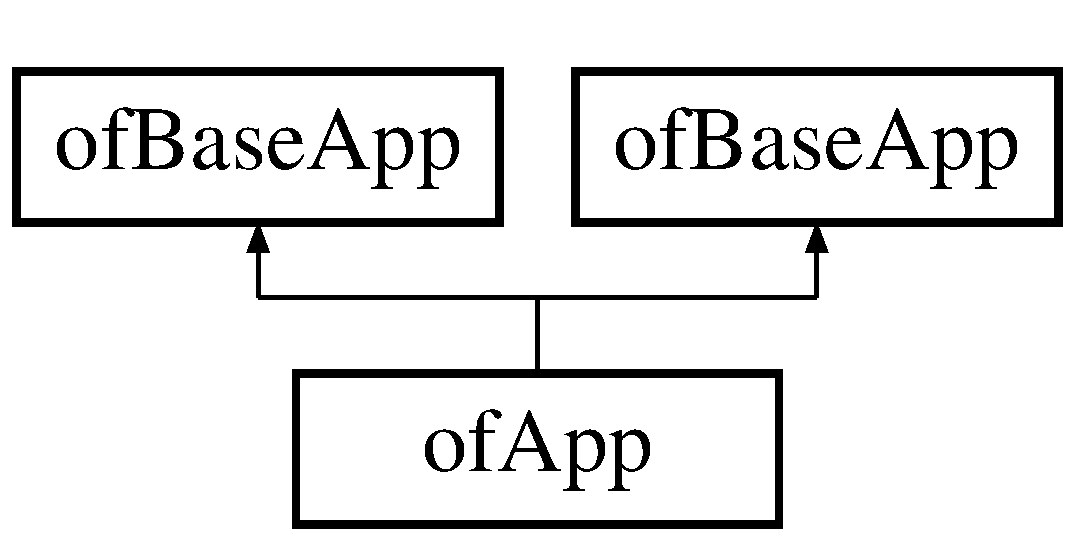
\includegraphics[height=2.000000cm]{classof_app}
\end{center}
\end{figure}
\subsection*{Public Types}
\begin{DoxyCompactItemize}
\item 
\hypertarget{classof_app_a1fa510985ab814a37d2a8cec474ef31f}{}enum {\bfseries esc} \{ \\*
{\bfseries inicio}, 
{\bfseries principal}, 
{\bfseries galeria}, 
{\bfseries inicio}, 
\\*
{\bfseries principal}, 
{\bfseries galeria}
 \}\label{classof_app_a1fa510985ab814a37d2a8cec474ef31f}

\item 
\hypertarget{classof_app_a1fa510985ab814a37d2a8cec474ef31f}{}enum {\bfseries esc} \{ \\*
{\bfseries inicio}, 
{\bfseries principal}, 
{\bfseries galeria}, 
{\bfseries inicio}, 
\\*
{\bfseries principal}, 
{\bfseries galeria}
 \}\label{classof_app_a1fa510985ab814a37d2a8cec474ef31f}

\end{DoxyCompactItemize}
\subsection*{Public Member Functions}
\begin{DoxyCompactItemize}
\item 
\hypertarget{classof_app_af68eaa1366244f7a541cd08e02199c12}{}void {\bfseries setup} ()\label{classof_app_af68eaa1366244f7a541cd08e02199c12}

\item 
\hypertarget{classof_app_afef41ea4aee5a22ea530afba33ae7a7b}{}void {\bfseries update} ()\label{classof_app_afef41ea4aee5a22ea530afba33ae7a7b}

\item 
\hypertarget{classof_app_a75dd45437b9e317db73d8daef1ad49f8}{}void {\bfseries draw} ()\label{classof_app_a75dd45437b9e317db73d8daef1ad49f8}

\item 
\hypertarget{classof_app_a957d3197364bbac8e67eaa4f15b28ad3}{}void {\bfseries key\+Pressed} (int key)\label{classof_app_a957d3197364bbac8e67eaa4f15b28ad3}

\item 
\hypertarget{classof_app_aa1503a87453bcfdd395fe4acca5d91a0}{}void {\bfseries key\+Released} (int key)\label{classof_app_aa1503a87453bcfdd395fe4acca5d91a0}

\item 
\hypertarget{classof_app_a158b41a606310db4633fdb817b21047c}{}void {\bfseries mouse\+Moved} (int x, int y)\label{classof_app_a158b41a606310db4633fdb817b21047c}

\item 
\hypertarget{classof_app_a1ec53d1be799dc275806ff6c6548cd83}{}void {\bfseries mouse\+Dragged} (int x, int y, int button)\label{classof_app_a1ec53d1be799dc275806ff6c6548cd83}

\item 
\hypertarget{classof_app_a2c2ea9c160231e55424dfd98466ef27d}{}void {\bfseries mouse\+Pressed} (int x, int y, int button)\label{classof_app_a2c2ea9c160231e55424dfd98466ef27d}

\item 
\hypertarget{classof_app_aa3131f1554fc49eaa9ee0f284e48129b}{}void {\bfseries mouse\+Released} (int x, int y, int button)\label{classof_app_aa3131f1554fc49eaa9ee0f284e48129b}

\item 
\hypertarget{classof_app_ae4dc1ec1513dcbe48bc78a5e4c3fac0f}{}void {\bfseries window\+Resized} (int w, int h)\label{classof_app_ae4dc1ec1513dcbe48bc78a5e4c3fac0f}

\item 
\hypertarget{classof_app_aada5a79556321801567752a0e5a69bda}{}void {\bfseries drag\+Event} (of\+Drag\+Info drag\+Info)\label{classof_app_aada5a79556321801567752a0e5a69bda}

\item 
\hypertarget{classof_app_a885672a72340a5e998af1d16718dc766}{}void {\bfseries got\+Message} (of\+Message msg)\label{classof_app_a885672a72340a5e998af1d16718dc766}

\item 
\hypertarget{classof_app_aa2a2572523fa300395395b1a7ec88e05}{}void {\bfseries estados\+Escenas} (bool, bool, bool)\label{classof_app_aa2a2572523fa300395395b1a7ec88e05}

\item 
\hypertarget{classof_app_a2a1b38d864089ce7aad3b04d13c72f0a}{}void {\bfseries sel\+Escena} (int)\label{classof_app_a2a1b38d864089ce7aad3b04d13c72f0a}

\item 
\hypertarget{classof_app_af68eaa1366244f7a541cd08e02199c12}{}void {\bfseries setup} ()\label{classof_app_af68eaa1366244f7a541cd08e02199c12}

\item 
\hypertarget{classof_app_afef41ea4aee5a22ea530afba33ae7a7b}{}void {\bfseries update} ()\label{classof_app_afef41ea4aee5a22ea530afba33ae7a7b}

\item 
\hypertarget{classof_app_a75dd45437b9e317db73d8daef1ad49f8}{}void {\bfseries draw} ()\label{classof_app_a75dd45437b9e317db73d8daef1ad49f8}

\item 
\hypertarget{classof_app_a957d3197364bbac8e67eaa4f15b28ad3}{}void {\bfseries key\+Pressed} (int key)\label{classof_app_a957d3197364bbac8e67eaa4f15b28ad3}

\item 
\hypertarget{classof_app_aa1503a87453bcfdd395fe4acca5d91a0}{}void {\bfseries key\+Released} (int key)\label{classof_app_aa1503a87453bcfdd395fe4acca5d91a0}

\item 
\hypertarget{classof_app_a158b41a606310db4633fdb817b21047c}{}void {\bfseries mouse\+Moved} (int x, int y)\label{classof_app_a158b41a606310db4633fdb817b21047c}

\item 
\hypertarget{classof_app_a1ec53d1be799dc275806ff6c6548cd83}{}void {\bfseries mouse\+Dragged} (int x, int y, int button)\label{classof_app_a1ec53d1be799dc275806ff6c6548cd83}

\item 
\hypertarget{classof_app_a2c2ea9c160231e55424dfd98466ef27d}{}void {\bfseries mouse\+Pressed} (int x, int y, int button)\label{classof_app_a2c2ea9c160231e55424dfd98466ef27d}

\item 
\hypertarget{classof_app_aa3131f1554fc49eaa9ee0f284e48129b}{}void {\bfseries mouse\+Released} (int x, int y, int button)\label{classof_app_aa3131f1554fc49eaa9ee0f284e48129b}

\item 
\hypertarget{classof_app_ae4dc1ec1513dcbe48bc78a5e4c3fac0f}{}void {\bfseries window\+Resized} (int w, int h)\label{classof_app_ae4dc1ec1513dcbe48bc78a5e4c3fac0f}

\item 
\hypertarget{classof_app_aada5a79556321801567752a0e5a69bda}{}void {\bfseries drag\+Event} (of\+Drag\+Info drag\+Info)\label{classof_app_aada5a79556321801567752a0e5a69bda}

\item 
\hypertarget{classof_app_a885672a72340a5e998af1d16718dc766}{}void {\bfseries got\+Message} (of\+Message msg)\label{classof_app_a885672a72340a5e998af1d16718dc766}

\item 
\hypertarget{classof_app_aa2a2572523fa300395395b1a7ec88e05}{}void {\bfseries estados\+Escenas} (bool, bool, bool)\label{classof_app_aa2a2572523fa300395395b1a7ec88e05}

\item 
\hypertarget{classof_app_a7fd7984af79ba9ba02726836cf6740df}{}void {\bfseries sel\+Escena} (int, string)\label{classof_app_a7fd7984af79ba9ba02726836cf6740df}

\item 
\hypertarget{classof_app_a7cc13ef3c1a4af65991a1bfd348de7fb}{}void {\bfseries rafaga} (bool, esc, string)\label{classof_app_a7cc13ef3c1a4af65991a1bfd348de7fb}

\end{DoxyCompactItemize}
\subsection*{Public Attributes}
\begin{DoxyCompactItemize}
\item 
\hypertarget{classof_app_ae769e8719339a6d9bea08d27471eec2c}{}enum of\+App\+::esc {\bfseries escenas}\label{classof_app_ae769e8719339a6d9bea08d27471eec2c}

\item 
\hypertarget{classof_app_a276986bf8ca05cc08ed99fa2c7a3aade}{}esc {\bfseries escena\+Sel}\label{classof_app_a276986bf8ca05cc08ed99fa2c7a3aade}

\item 
\hypertarget{classof_app_a28533eed35e42c643103cffe6947ee20}{}esc {\bfseries escena\+Rafaga}\label{classof_app_a28533eed35e42c643103cffe6947ee20}

\item 
\hypertarget{classof_app_a73dce5457705c30e2f46f3084dfcd9b7}{}ofx\+Tween {\bfseries tween}\label{classof_app_a73dce5457705c30e2f46f3084dfcd9b7}

\item 
\hypertarget{classof_app_a10b99ac9ad5f1219ff3076cbe560eb91}{}ofx\+Easing\+Linear {\bfseries easing}\label{classof_app_a10b99ac9ad5f1219ff3076cbe560eb91}

\end{DoxyCompactItemize}


The documentation for this class was generated from the following files\+:\begin{DoxyCompactItemize}
\item 
src/backup/of\+App.\+h\item 
src/backup/of\+App.\+cpp\end{DoxyCompactItemize}

\hypertarget{class_principal}{}\section{Principal Class Reference}
\label{class_principal}\index{Principal@{Principal}}
\subsection*{Public Member Functions}
\begin{DoxyCompactItemize}
\item 
\hypertarget{class_principal_a5f86602728685ff0321be8f97f45d339}{}void {\bfseries draw} (int \+\_\+r, int \+\_\+g, int \+\_\+b)\label{class_principal_a5f86602728685ff0321be8f97f45d339}

\item 
\hypertarget{class_principal_a9ded684f2e0f3c66cce1ce6ec37f63d8}{}void {\bfseries update} ()\label{class_principal_a9ded684f2e0f3c66cce1ce6ec37f63d8}

\item 
\hypertarget{class_principal_acd009737c79f22030d042200c483493f}{}void {\bfseries estados} (bool)\label{class_principal_acd009737c79f22030d042200c483493f}

\item 
\hypertarget{class_principal_a7c0ba9bd013645466da93eab75a7fd4b}{}void {\bfseries activar} ()\label{class_principal_a7c0ba9bd013645466da93eab75a7fd4b}

\item 
\hypertarget{class_principal_ae008133a15874968e0d9ea830f9adaf3}{}void {\bfseries desactivar} ()\label{class_principal_ae008133a15874968e0d9ea830f9adaf3}

\item 
\hypertarget{class_principal_aece6c65fb923c23e45f8e6102e845768}{}void {\bfseries iniciar} (string)\label{class_principal_aece6c65fb923c23e45f8e6102e845768}

\end{DoxyCompactItemize}
\subsection*{Public Attributes}
\begin{DoxyCompactItemize}
\item 
\hypertarget{class_principal_ac0011cd8fa717fd996392df849dd0703}{}bool {\bfseries boton\+Panel\+Activo}\label{class_principal_ac0011cd8fa717fd996392df849dd0703}

\item 
\hypertarget{class_principal_aafda82aa7c08c46ea313e02685201a5a}{}\hyperlink{classgestor3_d}{gestor3\+D} {\bfseries escena3\+D}\label{class_principal_aafda82aa7c08c46ea313e02685201a5a}

\item 
\hypertarget{class_principal_a891e0096a9d80bd9d20623613747e85e}{}of\+Light {\bfseries iluminacion}\label{class_principal_a891e0096a9d80bd9d20623613747e85e}

\item 
\hypertarget{class_principal_aac709415f2b6cbb4f477bea7f29f324a}{}\hyperlink{classboton}{boton} {\bfseries boton\+Panel}\label{class_principal_aac709415f2b6cbb4f477bea7f29f324a}

\item 
\hypertarget{class_principal_a6af3f1983a9640efc995e135e13d32e6}{}\hyperlink{classboton}{boton} {\bfseries btn\+Contenedor}\label{class_principal_a6af3f1983a9640efc995e135e13d32e6}

\item 
\hypertarget{class_principal_ac60ffbe7e2be3e6278562a409464334d}{}string {\bfseries titulo}\label{class_principal_ac60ffbe7e2be3e6278562a409464334d}

\item 
\hypertarget{class_principal_aec1a2c2811777c3649002dee5eaaa2a0}{}\hyperlink{class_contenedor}{Contenedor} {\bfseries gui\+Estatico}\label{class_principal_aec1a2c2811777c3649002dee5eaaa2a0}

\item 
\hypertarget{class_principal_aa7cb439e51bf95016c33175a7449b142}{}\hyperlink{classcaja_boton}{caja\+Boton} {\bfseries caja\+Btn}\label{class_principal_aa7cb439e51bf95016c33175a7449b142}

\item 
\hypertarget{class_principal_acd9deb3d7bc5c8deeb20cabd0bdce5d3}{}\hyperlink{classcaja_texto}{caja\+Texto} {\bfseries caja\+Txt}\label{class_principal_acd9deb3d7bc5c8deeb20cabd0bdce5d3}

\item 
\hypertarget{class_principal_a03f3c45162ef82d132a5f907dfc5324a}{}\hyperlink{classcaja_imagen}{caja\+Imagen} {\bfseries caja\+Img}\label{class_principal_a03f3c45162ef82d132a5f907dfc5324a}

\item 
\hypertarget{class_principal_a99a502ec7cf76b4d693e402296c2e8ed}{}\hyperlink{classcaja_gr_circulos}{caja\+Gr\+Circulos} {\bfseries caja\+Circulo}\label{class_principal_a99a502ec7cf76b4d693e402296c2e8ed}

\item 
\hypertarget{class_principal_a1cb34111059b2ac3d00f7e91e672a51b}{}\hyperlink{classcaja_gr_circulos}{caja\+Gr\+Circulos} {\bfseries otra\+Caja\+C}\label{class_principal_a1cb34111059b2ac3d00f7e91e672a51b}

\end{DoxyCompactItemize}


The documentation for this class was generated from the following files\+:\begin{DoxyCompactItemize}
\item 
src/\+Escenas/Principal.\+h\item 
src/\+Escenas/Principal.\+cpp\end{DoxyCompactItemize}

\hypertarget{class_rafaga}{}\section{Rafaga Class Reference}
\label{class_rafaga}\index{Rafaga@{Rafaga}}
\subsection*{Public Member Functions}
\begin{DoxyCompactItemize}
\item 
\hyperlink{class_rafaga_a9e01a40ca76ac95f9e3aec362b0cbbc0}{Rafaga} (float, float=500, of\+Color=of\+Color\+::light\+Gray)
\item 
\hypertarget{class_rafaga_a312a7d003583244f5da8cb6b2a49ff21}{}void {\bfseries draw} ()\label{class_rafaga_a312a7d003583244f5da8cb6b2a49ff21}

\item 
\hypertarget{class_rafaga_a6e97b28e4cbd2d31fe54ed6db2facf2a}{}void {\bfseries update} ()\label{class_rafaga_a6e97b28e4cbd2d31fe54ed6db2facf2a}

\item 
\hypertarget{class_rafaga_a54e4d7f24a8a35dc0d8fe23c33f5cf1f}{}void {\bfseries estado} (bool)\label{class_rafaga_a54e4d7f24a8a35dc0d8fe23c33f5cf1f}

\item 
\hypertarget{class_rafaga_a43adf6476f37cabffcc71f5a5234cf4b}{}bool {\bfseries getter} ()\label{class_rafaga_a43adf6476f37cabffcc71f5a5234cf4b}

\end{DoxyCompactItemize}
\subsection*{Public Attributes}
\begin{DoxyCompactItemize}
\item 
\hypertarget{class_rafaga_a080e63c4e672ff07a6578b9f67e6fd0c}{}bool {\bfseries iniciar}\label{class_rafaga_a080e63c4e672ff07a6578b9f67e6fd0c}

\item 
\hypertarget{class_rafaga_a65a915875cbd8e82512e15cc67998144}{}ofx\+Tween {\bfseries anim}\label{class_rafaga_a65a915875cbd8e82512e15cc67998144}

\item 
\hypertarget{class_rafaga_a73b5f84ddef001adb62f421a3ccd6306}{}ofx\+Tween {\bfseries anim\+Salida}\label{class_rafaga_a73b5f84ddef001adb62f421a3ccd6306}

\item 
\hypertarget{class_rafaga_a605a36c40458258beed83fa463528893}{}ofx\+Easing\+Quint {\bfseries Easing\+Sine}\label{class_rafaga_a605a36c40458258beed83fa463528893}

\item 
\hypertarget{class_rafaga_a14f2da7cec4e2186c788c3295a951978}{}\hyperlink{class_contenedor}{Contenedor} {\bfseries contenedor}\label{class_rafaga_a14f2da7cec4e2186c788c3295a951978}

\item 
\hypertarget{class_rafaga_a0451257813dedb044706cae5bac8aef7}{}\hyperlink{classcaja_imagen}{caja\+Imagen} {\bfseries caja\+Img}\label{class_rafaga_a0451257813dedb044706cae5bac8aef7}

\item 
\hypertarget{class_rafaga_a62e14e8b4b593b501a87ebfc4c5ef038}{}\hyperlink{classcaja_texto}{caja\+Texto} {\bfseries caja\+Txt}\label{class_rafaga_a62e14e8b4b593b501a87ebfc4c5ef038}

\end{DoxyCompactItemize}


\subsection{Constructor \& Destructor Documentation}
\hypertarget{class_rafaga_a9e01a40ca76ac95f9e3aec362b0cbbc0}{}\index{Rafaga@{Rafaga}!Rafaga@{Rafaga}}
\index{Rafaga@{Rafaga}!Rafaga@{Rafaga}}
\subsubsection[{Rafaga(float, float=500, of\+Color=of\+Color\+::light\+Gray)}]{\setlength{\rightskip}{0pt plus 5cm}Rafaga\+::\+Rafaga (
\begin{DoxyParamCaption}
\item[{float}]{\+\_\+duracion, }
\item[{float}]{\+\_\+velocidad = {\ttfamily 500}, }
\item[{of\+Color}]{\+\_\+color = {\ttfamily ofColor\+:\+:lightGray}}
\end{DoxyParamCaption}
)}\label{class_rafaga_a9e01a40ca76ac95f9e3aec362b0cbbc0}
prametros 
\begin{DoxyParams}{Parameters}
{\em duracion} & \\
\hline
{\em velocidad} & animacion (defecto 500) \\
\hline
{\em color} & de fondo (defecto light\+Gray) \\
\hline
\end{DoxyParams}


The documentation for this class was generated from the following files\+:\begin{DoxyCompactItemize}
\item 
src/Rafaga.\+h\item 
src/Rafaga.\+cpp\end{DoxyCompactItemize}

\hypertarget{class_titulo}{}\section{Titulo Class Reference}
\label{class_titulo}\index{Titulo@{Titulo}}
\subsection*{Public Member Functions}
\begin{DoxyCompactItemize}
\item 
\hypertarget{class_titulo_ad87b7f4b7b987cf1eefb682949dca844}{}void {\bfseries draw} ()\label{class_titulo_ad87b7f4b7b987cf1eefb682949dca844}

\item 
\hypertarget{class_titulo_a3fb7e8c49b7b414b1d4bee60f7c706d1}{}void {\bfseries update} ()\label{class_titulo_a3fb7e8c49b7b414b1d4bee60f7c706d1}

\item 
\hypertarget{class_titulo_adebe0d86f62e7e809912c00007f72d5f}{}void {\bfseries fbo\+Contenido} ()\label{class_titulo_adebe0d86f62e7e809912c00007f72d5f}

\item 
\hypertarget{class_titulo_a40fcb404b1162fab2b2cb87d864e867b}{}void {\bfseries animacion} ()\label{class_titulo_a40fcb404b1162fab2b2cb87d864e867b}

\item 
\hypertarget{class_titulo_a0ac8141c8e692d06a27916c82d9e7360}{}void {\bfseries setter} (string)\label{class_titulo_a0ac8141c8e692d06a27916c82d9e7360}

\end{DoxyCompactItemize}
\subsection*{Public Attributes}
\begin{DoxyCompactItemize}
\item 
\hypertarget{class_titulo_a11ed363267671e800063299568ecc9e9}{}float {\bfseries desplazamiento}\label{class_titulo_a11ed363267671e800063299568ecc9e9}

\item 
\hypertarget{class_titulo_aaa194e5e72a1242058dfdcee86a0f6ef}{}bool {\bfseries inicia\+Anim}\label{class_titulo_aaa194e5e72a1242058dfdcee86a0f6ef}

\item 
\hypertarget{class_titulo_a00c81b1c73caa62cf9ac9b0ea7da1247}{}of\+True\+Type\+Font {\bfseries titulo}\label{class_titulo_a00c81b1c73caa62cf9ac9b0ea7da1247}

\item 
\hypertarget{class_titulo_a5abfcc1d2c4831305cced64593c9b339}{}string {\bfseries texto\+Titulo}\label{class_titulo_a5abfcc1d2c4831305cced64593c9b339}

\item 
\hypertarget{class_titulo_a49b321e3499b0013a7767f5e94493e26}{}string {\bfseries stack}\label{class_titulo_a49b321e3499b0013a7767f5e94493e26}

\item 
\hypertarget{class_titulo_a11953b36202597438f89287ded91f4d5}{}of\+Fbo {\bfseries Fbo\+Caja}\label{class_titulo_a11953b36202597438f89287ded91f4d5}

\item 
\hypertarget{class_titulo_a739731c069e3143f35eac3e103f00f58}{}ofx\+Tween {\bfseries animacion\+Titulo}\label{class_titulo_a739731c069e3143f35eac3e103f00f58}

\item 
\hypertarget{class_titulo_a703efa8ca1c9d6a0b13072f803c5ec44}{}ofx\+Easing\+Back {\bfseries easing}\label{class_titulo_a703efa8ca1c9d6a0b13072f803c5ec44}

\end{DoxyCompactItemize}


The documentation for this class was generated from the following files\+:\begin{DoxyCompactItemize}
\item 
src/\+Gui/Titulo.\+h\item 
src/\+Gui/Titulo.\+cpp\end{DoxyCompactItemize}

%--- End generated contents ---

% Index
\backmatter
\newpage
\phantomsection
\clearemptydoublepage
\addcontentsline{toc}{chapter}{Index}
\printindex

\end{document}
